\documentclass[final]{svjour2}
\usepackage{amsmath}
\usepackage{graphicx}
\usepackage{rotating}
\usepackage{amssymb}
\usepackage{mathptmx}
\usepackage[numbers]{natbib}
\usepackage{float}
\usepackage[section]{placeins}
\usepackage{tabularx}
\usepackage{booktabs}
\usepackage{color}
\usepackage{epstopdf}
\usepackage[table]{xcolor}
\usepackage{threeparttable}

\makeatletter
\journalname{Journal of Low Temperature Physics}
%%%%%%%%%%%%%%%%%%%%%%%%%%%%%% Textclass specific LaTeX commands.
%%%%%%%%%%%%%%%%%%%%%%%%%%%%%% User specified LaTeX commands.
\bibpunct{}{}{,}{s}{}{,}

\begin{document}

\newcommand{\hdblarrow}{H\makebox[0.9ex][l]{$\downdownarrows$}-}
\title{Material Selection for Cryogenic Support Structures}

\author{E. Kramer \and N. Kellaris  \and M. Daal  \and B. Sadoulet \and S. Golwala \and M. Hollister}

\institute{Department of Physics, U.C. Berkeley,\\ Berkeley, CA 94709, USA\\
\email{ekramer@berkeley.edu}}

\date{08.02.2013}

\maketitle

\begin{abstract}

Design specifications for the support structures of low temperature instrumentation often call for low thermal conductivity between temperature stages, high stiffness, and specific load bearing capabilities.  While overall geometric design plays an important role in both overall stiffness and heat conduction between stages, material selection can affect a structure's properties significantly.  In this contribution, we suggest and compare several alternative materials to the current standard materials for building cryogenic support structures.

\keywords{Cryogenic, Low Temperature, Cryogenic Materials, Thermal Conductivity, Material Strength, Young's Modulus, Cryogenic Support, Support Structures, Truss, Structural Materials}

\end{abstract}

\section{Introduction}
Cryogenic support structures are typically engineered to meet three design specifications: low thermal conductance, high strength, and high stiffness. Creating support structures that obtain the lowest thermal conductance between temperature stages while still remaining structurally adequate to support forces imposed during operation at base temperature and handling at room temperature is a design optimization problem. The thermal consideration usually results in structures suspended by elements possessing minimized cross-sectional area such as thin plates, webs of yarn, slender rods or tubes. The application will dictate which parameter, strength or stiffness, imposes the next most limiting design constraint. Focusing on the case of stiffness, we draw attention to the fact that both stiffness and power conducted are proportional to the cross-sectional area, $A$, divided by the length, $l$, of the structure support members.\cite{Hastings1993} As we will explain, this provides a helpful parameterization for the selection of cryogenic support structural materials.

\section{Material Selection and Design Parameters}

The property that is primarily used to describe the stiffness or elasticity of a material is its Young's modulus. Young's modulus is formally defined for tensile stresses, but for isotropic materials one can extend the notion for use with compressive forces. Young's Modulus is sometimes called the {\em elastic modulus} or {\em modulus of elasticity}. It is the ratio of the stress along a given axis over the strain along the same axis in the range of values where Hooke's law holds\footnote{Stress ($\sigma$) here is defined as the force applied in the direction normal to a sample's cross section divided by the cross sectional area of the sample (assuming a constant cross sectional area) $\sigma = F/A_{0}$.  Strain ($\epsilon$) is defined as the change in length of the sample in the direction of the applied force over the original length $\epsilon=\Delta L/L_{0}$.}.  Young's modulus can sometimes be different for tensile stress (the {\em tensile modulus}) and the compressive stress (the {\em compressive modulus})\footnote{When tensile and compressive moduli are not equal this is due to an asymmetry (e.g. the specimen is a string), or a rapid variation of the modulus which occurs through zero strain, but this is not a discontinuity in the curve. Materials exhibiting this rapid change in modulus around zero stress are called {\em bimodulus} or {\em bilinear} materials.}. It should also be pointed out that different samples of the same material may have different moduli as a result of their defect characteristics, heat treatments, etc.

\begin{table}[htb]%THERMOPHYSICAL PROPERTIES
\begin{threeparttable}
\rowcolors{3}{gray!20}{white}
\begin{tabular}{lrrrrrr}
\toprule
\textbf{Material} & $\rho$ ($\frac{g}{cm^3}$) & $\nu$ & $\sigma_{t}$ (MPa) & $\sigma_{c}$ (MPa) & TM (GPa) & CM (CPa) \\
\midrule
 POCO AXM-5Q & 1.73 & 0.27 & 48\tnote{U} & 124\tnote{U} & 10.5 & - \\
 TIMET Ti 15-3-3-3 & 4.78 & 0.36 & 766\tnote{Y} & 810\tnote{Y} & 82.0 & 90.0\\
 Stainless 316LN & 7.99 & 0.29 & 690\tnote{Y} & - & 200.0 & - \\
 Vespel SP-1 & 1.43 & 0.41 & 86 & 133\tnote{*} & 2.5\tnote{\dag} & 2.4 \\
 Vespel SCP-5000 & 1.46 & - & 163 & 230\tnote{*} & 4.0 & 9.1 \\
 Vespel SP-22 & 1.65 & - & 52 & 112\tnote{*} & 2.5 & 3.3 \\
 Vespel SCP-5050 & 1.76 & 0.22 & 72 & 172\tnote{*} & 8.9 & 3.0 \\
 Torlon 4301 & 1.46 & - & 113\tnote{U} & 166\tnote{U} & 6.8 & 5.3 \\
 G-10CR & 1.90 & 0.18 & 429\tnote{U} & 374\tnote{U} & 27.9 & 15.0 \\
 Graphlite CF Rod & 1.55 & -  & 2340 & 1900 & 134.0 & 131.0 \\
 Kevlar 49 Fibers & 1.44 & 0.36 & 3000\tnote{U} & - & 112.4 & - \\
 Macor & 2.52 & 0.29 & 90\tnote{U} & 345\tnote{U} & 66.9 & 64.0 \\

 \bottomrule
\end{tabular}
\caption{Some physical and mechanical properties of candidate materials. $\nu$ is the Poisson's ratio for the material, while $\sigma_{t}$ and $\sigma_{c}$ are the tensile and compressive strengths for the material, respectively. Superscripts on strengths refer to: Y - yield strength, U - ultimate strength, * - compressive load at \%10 strain. Unmarked numbers have unknown failure conditions. TM and CM are the tensile and compressive elastic moduli respectively. A blank indicates that the specified property could not be found in the literature for a given material. Data comes largely from manufacturer's literature; where values were missing from manufacturer literature, outside references were used; references as well as relevant notes about the material properties are as follows: POCO AXM-5Q -- $\nu$ from \cite{Swank2009}; Ti 15-3-3-3 -- $\nu$, $\sigma_t$, $\sigma_c$, CM from \cite{Lang2001}\cite{Johnson1996}\cite{Nyakana2005}. All properties were for solution-treated material; SS316LN -- $\nu$ from \cite{Shankar2001}. Other data are from SS316LN data sheet for cold worked material (www.finetubes.com); Vespel -- TM for SP-1 from \cite{Doty1981}. All data were for isostatically formed parts. $\dag$ - Tensile modulus estimated from manufacturer's stress-strain plot; G-10CR -- all data from \cite{Kasen1981}\cite{Markley1985}. Properties taken in the warp direction; Graphlite CFRP -- properties along the fiber axis; Kevlar 49 -- all data are for unfilled fibers; Macor -- $\sigma_t$ and CM from \cite{Markley1985}\cite{websiteMacor}.}
\label{SW}
\end{threeparttable}
\end{table}

Except for yarn webbings, when loading a cryogenic support structure, the forces experienced generally tend to be of the same magnitude in both compressive and tensile directions.  Because of this, the smaller of the two moduli, the tensile modulus or the compressive modulus, must be focused on in order to keep a sufficient factor of safety and prevent premature failure.

It is also important to note the other properties of the material being used.  Ductile materials, such as most metals, tend to fail from shear forces first, while brittle materials like carbon fibers fail from normal forces first.  Another aspect of material selection is that of metallic versus non-metallic support. Metallic supports can be quite stiff, however they are not ideal for applications requiring electrically isolated stages.  Also, The shape of the thermal conductivity curve plays an important role as steep thermal conductivity curves create susceptibility to thermal run-aways in the cryostat.

Overall, when deciding on materials, they must be stiff enough to not fail under expected loads ranges while keeping their cross section is low as possible to minimize the amount of heat transfer between temperature stages. Because stiffness and power conducted are both proportional to the cross-sectional area divided by the length \footnote{The common $A/L$ dependence holds for small axial and radial loads. Other loads, such as off axis moments may not have this dependence and may result in structural weaknesses including reduced stiffness.}, $A/l$, we can normalize the Young's modulus of a material by its thermal conductivity in order to compare multiple materials for use in these structures. Runyan\cite{Runyan2008} et al. presented a very similar plot comparing different materials not featured in this contribution.  In general, because a high stiffness and low thermal conductance is typically desired, when choosing materials we want the smallest thermal conductivity to Young's Modulus ratio\cite{Hastings1993}. In the following plot we present a few newer useful materials along with familiar standbys that have the desired low thermal conductivity to Young's Modulus ratio.

\begin{figure}[ht]
\begin{center}
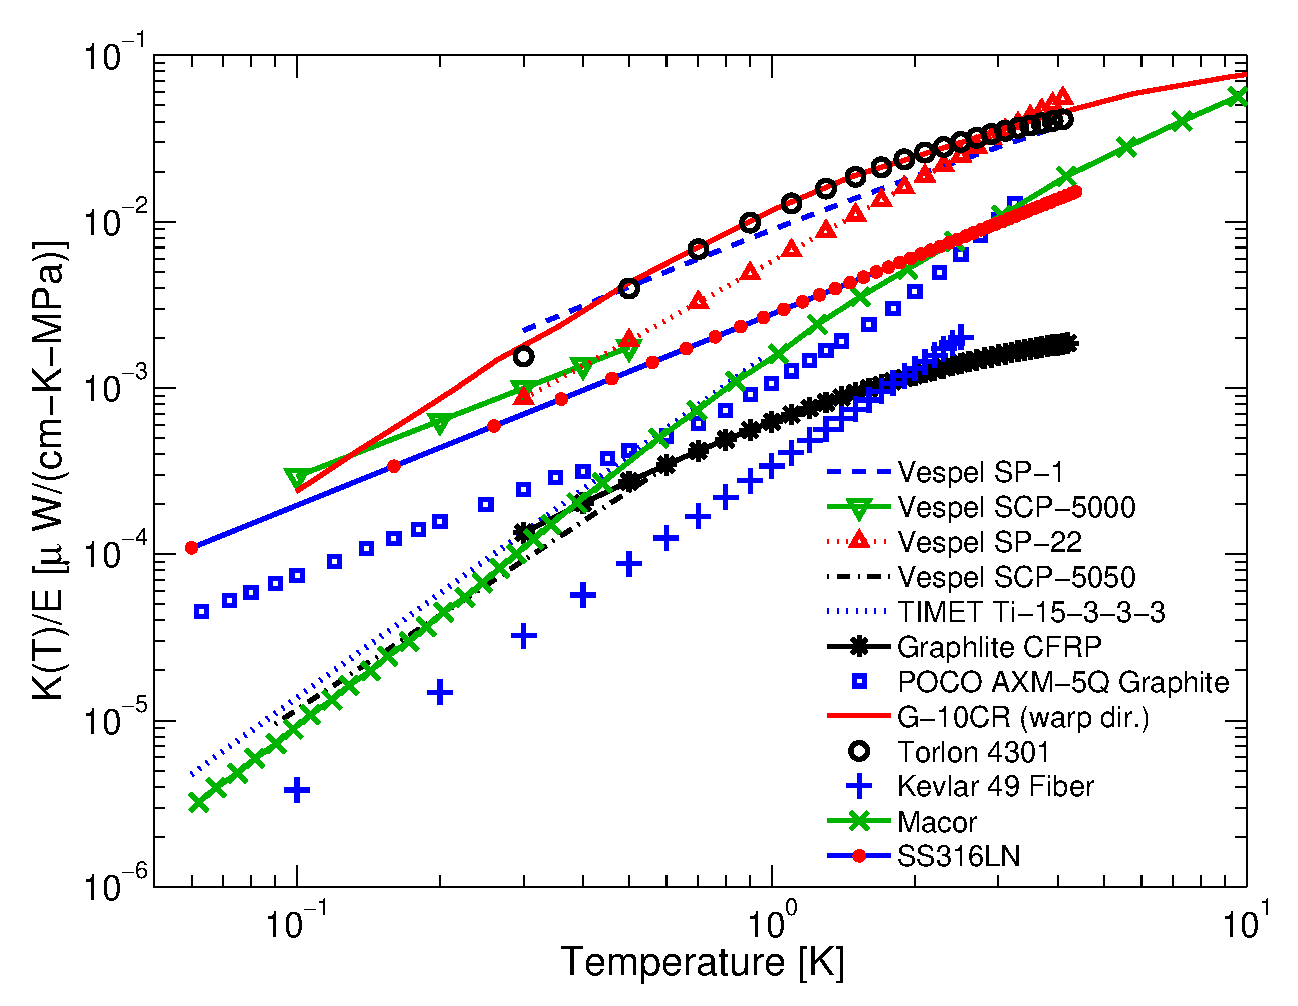
\includegraphics[%
  width=1\linewidth,
  keepaspectratio]{E_norm_support_K.eps}
\end{center}
\caption{A selection of useful materials with their room temperature Young's modulus normalized by their thermal conductivity.  Lower values are desirable as support materials.  Thermal conductivity references: Vespel SP-1, Vespel SP-22, Graphlite CFRP, and Torlon 4301 from Runyan\cite{Runyan2008}; Vespel SCP-5000, Vespel SCP-5050, and Ti 15-3-3-3 (under 20\% cold work after anneal) from Kellaris\cite{Kellaris2013}; AXM-5Q, G-10CR, and Macor from Woodcraft\cite{Woodcraft2009} \cite{Woodcraft2009_2}; Kevlar 49 from Ventura\cite{Ventura2009}; Stainless Steel 316LN from Barucci\cite{Barucci2008}. Young's moduli from table above.}
\label{Mats}
\end{figure}


\section{Conclusions}
While many different geometric design solutions exist, once the geometric design of a cryogenic support has been selected, the materials used to build it determine its strength, stiffness, and thermal conductance. A parameter useful in material selection is the material's thermal conductivity normalized to its Young's Modulus.  Unlike design geometry alterations, a change of material used to build a structure tends to be a much easier and predictable way to improve upon a design in terms of its performance under a force or heat load. Also, changes in material of a structure have the advantage of avoiding the necessity to make changes in the governing equations or model for theoretical evaluation due to the fact that material properties tend to be well defined dependent variables in both. For geometric designs that already exist and cannot be altered, a judicious change of support material using the data presented here could improve performance without necessarily entailing further detailed modeling.

\begin{acknowledgements}
We would like to thank Dr. Sanjay Govindjee of UC Berkeley for technical assistance. We acknowledge support and funding from the Department of Energy and the National Science Foundation.
\end{acknowledgements}

\begin{thebibliography}{99}

%%%%%%%%% Structure bibliography items %%%%%%%%%%
%%%%%%%%%%%%%%%%%%%%%%%%%%%%%%%%%%%%%%%%%%%%%%%%%
\bibitem{Hastings1993}
Peter R. Hastings and D.M. Montgomery, {\it Support of cooled components in astronomical instruments. Cryogenics} \textbf{2633(11)}, 1032 (1993).

\bibitem{Jenkins2005}
C. Jenkins and S. Khanna, {\it Mechanics of Materials: A Modern Integration of Mechanics and Materials in Structural Design} (Elsevier Academic Press, Burlington, MA, 2005).


%%%%%% Material Properties bibliography items %%%%%%%%%
%%%%%%%%%%%%%%%%%%%%%%%%%%%%%%%%%%%%%%%%%%%%%%%%%%%

%%% POCO-AXM5Q references
\bibitem{Swank2009}
D. Swank, W. Windes, D.C. Haggard, D. Rohrbaugh, and K. Moore, {\it Report prepared for the U.S. Dept. of Energy}. March 2009. INL/EXT-09-15515.

%%% Ti 15-3-3-3 references
\bibitem{Lang2001}
R. Lang, K. Hofmann, and H. Gese, {\it RTO Meeting Proceedings} \textbf{69(II)}. Loen, Norway, 7-11 May 2001.

\bibitem{Johnson1996}
W.S. Johnson, E. Li, and J.L. Miller, {\it Applied Composite Materials} \textbf{3}, 379 (1996).

\bibitem{Nyakana2005}
S.L. Nyakana, J.C. Fanning, and R.R. Boyer, {\it Journal of Materials Engineering and Performance} \textbf{14}, 799 (2005).

%%% Stainless Steel 316LN
\bibitem{Shankar2001}
P. Shankar, P. Palanichamy, T. Jayakumar, B. Raj, and S. Ranganathan, {\it Metallurgical and Materials Transactions A} \textbf{32A} 2960 (2001).

%%% Vespel SP-1
\bibitem{Doty1981}
F.D. Doty and P.D. Ellis, {\it Rev. Sci. Instrum.} \textbf{52(12)}, 1868, (1981).

%%% G-10CR
\bibitem{Kasen1981}
M.B. Kasen, G.R. MacDonald, D.H. Beekman, Jr., and R.E. Schramm, {\it Advances in Cryogenic Engineering Materials} \textbf{26}, 235, (1981).

%%% G-10CR & Macor
\bibitem{Markley1985}
F.W. Markley, J.A. Hoffman, and D.P. Muniz, {\it Cryo. Eng. Conference and Int. Cryo. Materials Conference}. Cambridge, MA, 12-16 August 1985.

%%% Macor
\bibitem{websiteMacor}
Ferro-Ceramic Grinding Inc. (http://www.ferroceramic.com/macor\_table.htm).

%%%% Thermal conductivity bibliography items %%%%
%%%%%%%%%%%%%%%%%%%%%%%%%%%%%%%%%%%%%%%%%%%%%%%%%

%%% Vespel SP-1, Vespel SP-22, Graphlite CFRP, Torlon 4301
\bibitem{Runyan2008}
M.C. Runyan and W.C. Jones, {\it Cryogenics} \textbf{48}, 448, (2008).

%%% Vespel SCP-5000, Vespel SCP-5050, Ti 15-3-3-3
\bibitem{Kellaris2013}
N.A. Kellaris. {\it Unpublished thermal conductivity measurements}, (2013).

%%% AXM-5Q
\bibitem{Woodcraft2009}
A.L. Woodcraft, M. Barucci, P.R. Hastings, L. Lolli, V. Martelli, L. Risegari, and G. Ventura, {\it Cryogenics} \textbf{49}, 159, (2009).

%%% G-10CR & Macor
\bibitem{Woodcraft2009_2}
A.L. Woodcraft and A. Gray, {\it Low Temp. Detectors 13, Proceedings of the 13$^{th}$ International Workshop} \textbf{1185}, 681, (2009).

%%% Kevlar 49
\bibitem{Ventura2009}
G. Ventura and V. Martelli, {\it Cryogenics} \textbf{49}, 376, (2009).

%%% Stainless Steel 316LN
\bibitem{Barucci2008}
M. Barucci, L. Lolli, L. Risegari, and G. Ventura, {\it Cryogenics} \textbf{48}, 166, (2008).

\end{thebibliography}

\end{document}
